The accuracy of the predictions of the thermo-electrical model is affected by two major factors: the quality of the input parameters, and the error introduced by reducing the complex 3D geometry into a linear thermal impedance network. The former has been discussed throughout this paper where the different inputs have been presented. For the latter, we have studied the agreement of predictions from the network model with the more accurate results obtained from FEA for selected states of the system.

To verify the level of this agreement, we have calculated the sensor temperature curve for a barrel EOS-type module up to thermal runaway, both in the full FEA and in the network model. For this exercise, we do not vary any of the input parameters in the model other than the sensor leakage power with its temperature dependence. The resistor values in the network model are the same as used throughout for our model, obtained as described in Section~\ref{sec:impedances}. For the power from the various electronics components, the FEAST efficiency and the TID scale factor we have used representative nominal values.

Because the variable model inputs are kept constant for this study, we can reduce the complex thermal network to its Th\'{e}venin equivalent, which is identical to the network studied in Ref.~\cite{Beck:2010zzd}, and use the analytical expressions given there. The reduced network is described by the base temperature $T_0$, defined as the sum of the coolant temperature and the temperature rise due to the front-end electronics alone, and the total thermal impedance $R_t$ from the sensor to the coolant. Using the nominal resistances and representative power numbers from the module, $T_0=-21.9~^\circ$C and $R_t=1.132$~K/W in the network model, compared to $-22.4~^\circ$C and 1.147~K/W obtained directly from the FEA. The comparison of the predicted sensor temperatures for both cases is shown in Fig.~\ref{fig:verification}. Despite a large temperature variation of about 10~$^\circ$C across the sensor, the network model runaway prediction agrees well with the FEA\footnote{The critical temperature here is $-12.4~^\circ$C, which is higher than the numbers given in Section~\ref{sec:systemprop}, because the study here ignores temperature effects such as the FEAST efficiency, which can only be modelled in the network model.}. This gives us confidence that the use of a thermal network model is not likely to significantly degrade the predictions beyond the uncertainties introduced by other inputs to the model. 

\begin{figure}[ht]
\centering
\subfloat[] {\label{fig:verification_a} 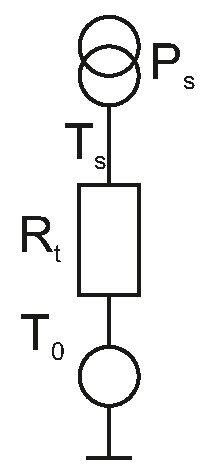
\includegraphics[width=0.11\linewidth,valign=c]{figures/replacement.pdf}}\quad
\subfloat[] {\label{fig:verification_b} 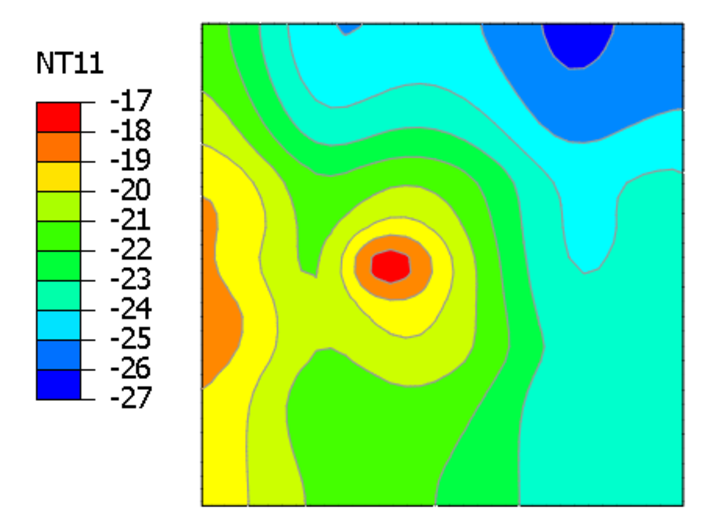
\includegraphics[width=0.32\linewidth,valign=c]{figures/verificationFEA.pdf}}\quad\quad
\subfloat[] {\label{fig:verification_c} 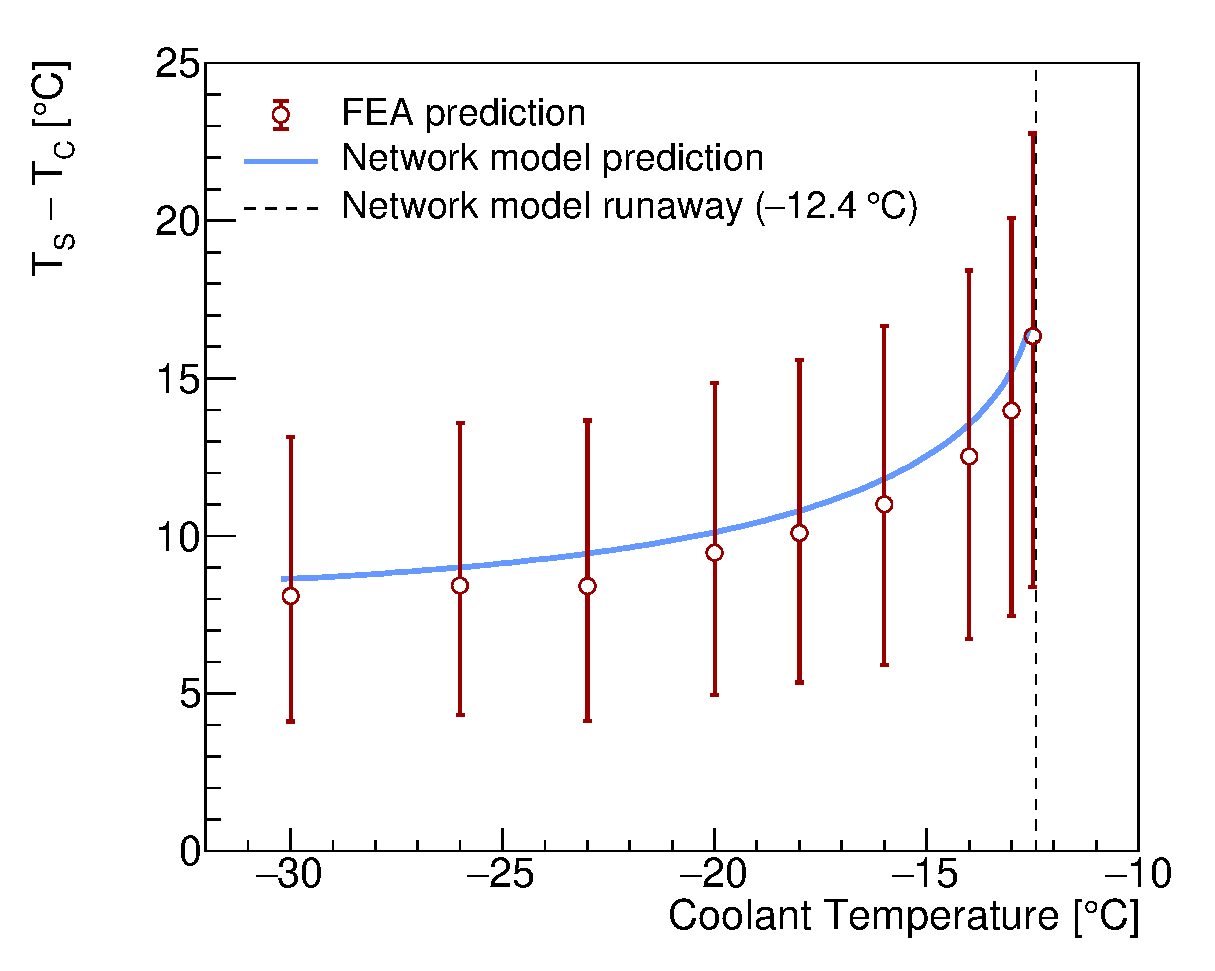
\includegraphics[width=0.45\linewidth,valign=c]{figures/verification_v2.eps}}
\caption{(a) Th\'{e}venin equivalent of the thermal network. (b) Result of sensor surface temperature calculations using FEA, assuming zero sensor power. The EOS card is to the left of the module, and the cooling pipes run from top to bottom about a quarter of the module width from each edge. The figure uses a rainbow colour gradient, with blue indicating the lowest temperatures and red the highest temperatures. (c) Difference of average sensor and coolant temperature, comparing FEA (red points) and the network model prediction (blue curve). The bars on the FEA data indicate minimum and maximum sensor temperature. The dotted vertical line indicates the critical temperature derived analytically using the network model ($-12.4~^\circ$C).}
\label{fig:verification}
\end{figure}
